\chapter{Experiments and results}

This chapter describes the experiments we performed to show the effectiveness of the proposed method. 

\section{Evaluation datasets}
To quantitatively evaluate the proposed methods, and to compare it to related work,
we considered two datasets: the DSO-1 and DSI-1 datasets\footnote{Public available for download at https://recodbr.wordpress.com/code-n-data}. Each dataset comes with a face position groundtruth and a splicing mask. Additionally, the ColorChecker dataset \cite{gehler2008bayesian} is used as a source of pristine images.


This dataset has been mainly used for experimenting on pristine data: due its characteristics is very varied and lends itself well to image analysis based on color.

\subsection{DSO-1}

The DSO-1 dataset is composed of 200 indoor and outdoor images with image resolution of 2048 × 1536 pixels. Out of this set of images, 100 are original, i. e., have no adjustments whatsoever, and 100 are forged. 

\begin{figure}[h!]
  \centering
    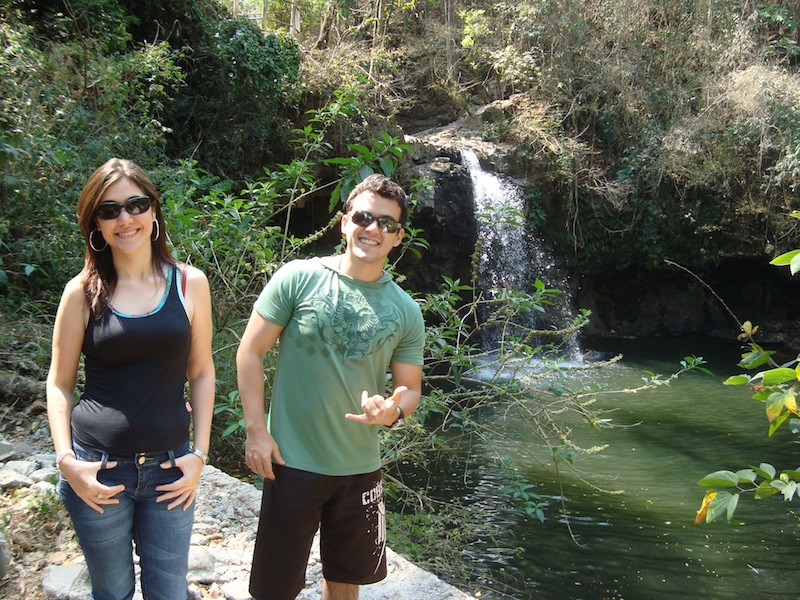
\includegraphics[width=0.65\textwidth]{dso1_sample}
    \caption{Example of an image of the DSO-1 dataset}
    \label{fig:dsosample}
\end{figure}

The forgeries were created by adding one or more individuals in a source image that already contained one or more people. When necessary, we complemented an image splicing operation with post-processing operations (such as color and brightness adjustments) in order to increase photorealism.

\subsection{DSI-1}

The DSI-1 dataset is composed of 50 images (25 original and 25 doctored) downloaded from different websites in the Internet with different resolutions. Original images were downloaded from Flickr and doctored images were collected from different websites such as Worth 1000, Benetton Group 2011, Planet Hiltron, etc.

\begin{figure}[h!]
  \centering
    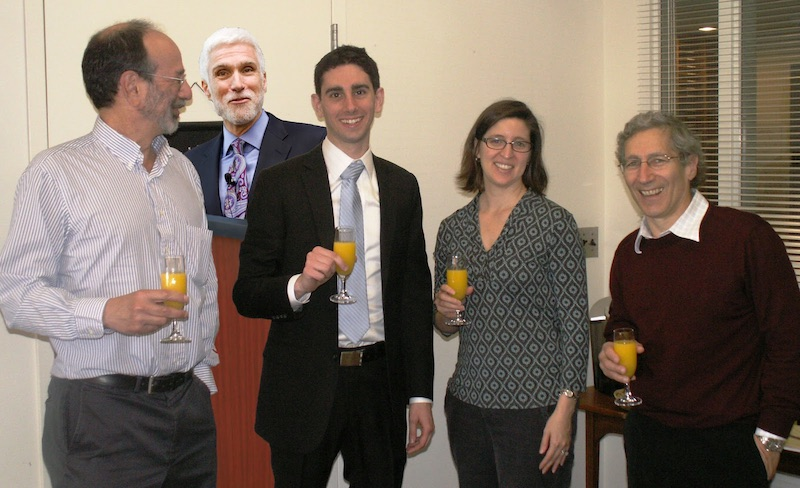
\includegraphics[width=0.65\textwidth]{dsi1_sample}
    \caption{Example of an image of the DSI-1 dataset}
    \label{fig:dsisample}
\end{figure}

\subsection{Colorchecker}

The ColorChecker dataset is a collection of images for evaluating Color Constancy algorithms built as additional material to \cite{gehler2008bayesian}. It consists in 568 RGB colored images of different scenes, both indoor and outdoor taken under different illuminations. In each scene a Gretag MacBeth Color Checker Chart was placed such that it was illuminated by the main scene illuminant and thus its color could be retrieved. The data is available in Canon RAW format free of any correction.

\begin{figure}[h!]
  \centering
    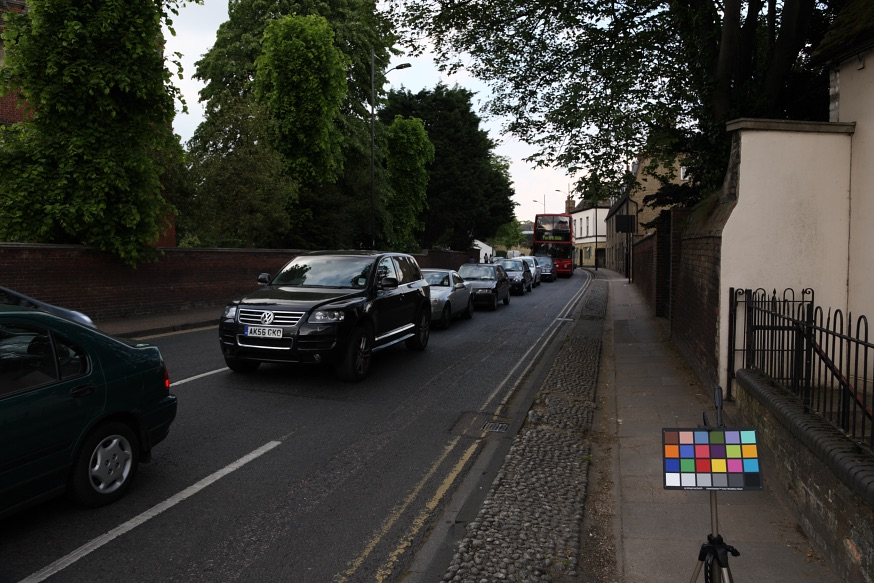
\includegraphics[width=0.65\textwidth]{colorchecker_sample}
    \caption{Example of an image of the ColorChecker dataset}
    \label{fig:colorcheckersample}
\end{figure}

\section{Face forgery detection module performance}

This section describes the experiments performed to evaluate the face forgery detection module. In these experiments, the DSO-1 and the DSI-1 datasets are used for evaluation.

In the classification stage, we used a 10-fold cross validation protocol, an SVM classifier with an RBF
kernel, and classical grid search for adjusting parameters in training samples \cite{bishop2007pattern}.

Experimental results are collected in Table \ref{table:performancefacedet}. 

\begin{table}[h!]
\caption{Performance of face forgery detection module over paired faces}
\label{table:performancefacedet}
\centering
\small
\begin{tabular}{l c c c c c} 
\hline \hline 
Test case & Train & Test & ACC & AUC & F-Score \\ [0.5ex]
\hline
Test 1 & DSO-1 & DSO-1 &	0.82 & 0.88	& 0.77\\
Test 2 & DSI-1 & DSI-1 &	0.87 & 0.92 & 0.87\\
Test 3 &	DSO-1 &	DSI-1 &	0.58 & 0.58 & 0.62\\
Test 4 &	DSI-1 & DSO-1 & 0.62 & 0.59 & 0.53\\ [1ex]
\hline
\end{tabular}
\end{table}


\subsection{Performance on DSO-1 dataset}

In this experiment, the proposed method has been applied to the DSO-1 dataset for classyfing paired faces as fake or real.





We now apply the proposed method for classifying an image as fake or real (the actual detection/
localization of the forgery shall be explored in Section 5.3.5). For this experiment,
we consider the DSO-1 dataset.



We have used the 10-fold cross-validation protocol for experiments over the same datasets.






Vengono di seguito presentati i risultati relativi alle performance del modulo di face detection forgeries su coppie di facce.

Per ciascuno dei casi di test presenti nella tabella vengono riportati:

	Il dataset su cui è stato fatto il training
	Il dataset su cui è stato effettuato il test
	Il valore di accuratezza (ACC) raggiunta nella classificazione
	Il valore dell’area sottesa alla curva ROC (AUC)
	Il valore di accuracy espresso in F1-Score (F-Score)


$$F_1=2*(precision*recall)/(precision+recall)$$


Per ciascun test sono allegati i file Matlab contenenti le labels e gli scores necessari per replicare i risultati della tabella.


I risultati portati in precedenza erano dati da una classificazione con votazione a maggioranza secca, in cui ciascun classificatore (degli otto totali) votava con 0 o 1 (a seconda della predizione). Gli scores qui considerati sono invece il risultato della somma di predizioni soft in [0, 1], in cui il singolo valore indica la confidenza della classificazione.

I risultati nella tabella sono dati dalla media aritmetica su 5 run dell’algoritmo.

\section{Regions forgery detection module performance}



